
\documentclass[letterpaper, 11pt]{report}
\usepackage{titlesec}
\usepackage{fullpage} % changes the margin
\usepackage{amsmath}
\usepackage{amssymb}
\usepackage{graphicx} %package to manage images
\usepackage[linkcolor=red]{hyperref}
\usepackage{paralist}
\usepackage{subcaption}
\usepackage{hyperref}
\graphicspath{ {./images/} }

\begin{document}
\begin{titlepage}
\vspace*{0.7in}
\begin{center}
\begin{figure}[htb]
\begin{center}

\includegraphics[width=9cm]{D1-Reengineering Opportunity/images/univ_logo.png}
\end{center}
\end{figure}
\vspace*{0.3in}
\begin{Large}
\textbf{SOEN 6431 : SOFTWARE COMPREHENSION AND MAINTENANCE} \\
\end{Large}
\vspace*{0.1in}
\begin{Large}
\textbf{Summer 2022} \\
\end{Large}
\vspace*{0.9in}
\begin{Large}
\textbf{Deliverable - 3 : Reengineering Outreach} \\
\href{https://github.com/manimayan/SOEN_6431_Deja_Vu}{Github Link}\\
\end{Large}
\vspace*{0.75in}
\begin{Large}
\textbf{\emph{Authors}} \\
\vspace*{0.2in}
Manimaran Palani\\
Iphigenia Pappas\\
Heet Patel\\
Kevinkumar Patel\\
Venis Patel \\
\end{Large}
\end{center}
\begin{center}
\vspace*{0.9in}
https://www.overleaf.com/project/610304de4e6b8d24f7c781b6\end{center}
\end{titlepage}

\tableofcontents
\newpage
\addcontentsline{toc}{section}{1. Abstract}
\section*{1. Abstract}
\normalsize { For a software system to be able to successfully sustain in the market, constant evolution becomes of utmost importance. Evolution refers to continuous developments and updates in the originally created software system to match the ever-changing market demands at any given point of time. This process of refining the software to keep it abreast of the trends and demands is termed as Software Maintenance. To carry out a successful maintenance by implementing positive changes in the software systems, the analysis of source code and documentation and having a comprehensive understanding of the system holds the most importance.\\

For this assignment, we choose a candidate R from five different repositories chosen by respective team members. We dive into the detailed analysis of the ‘undesirables’ in the repositories using TeamScale before tapering down to the candidate R. We further explain the repudiation rationale for the same. The chosen candidate R provides us with the opportunity to reengineer the software program by rectifying the ‘undesirables’ and thus improving its efficiency and maintainability.
}

\addcontentsline{toc}{section}{2. Introduction}
\section*{2. Introduction}
\normalsize {Software Maintenance plays a massive role in always keeping the software in a ‘good shape’. This inturn benefits the maintainers of the software in by-passing the whole cost and hassle of creating a new software system from scratch after being outdated and also aids in keeping it up-to-date according to the market needs. Maintenance also ensures solid quality of code and maintainability. This is very useful in safeguarding the software system from having potential ‘undesirables’ which can further lead to a decline in quality and efficiency of the source code.\\

A reengineering process on the source code and documentation of a software can further widen the horizon for itself in terms of its usability, maintainability and efficiency. We carry out an initial analysis using TeamScale of five different repositories by taking note of  five unique ‘undesirables’ for each one of them. We then analyze, based on the quality of the source code and documentation, the reasons for a repository to be an ideal candidate R for reengineering. \\

Upon successful identification of the candidate R, we buckle down to investigating the ‘undesirables’ in more detail. We further plan on materializing the solutions to the problems observed in the candidate R by carrying out reengineering operationalization in the upcoming assignment.}

\addcontentsline{toc}{section}{3. Project Deliberation}
\section*{3. Project Deliberation}
\addcontentsline{toc}{subsection}{3.1. Communal Work and Responsibility Matrix}
\subsubsection*{3.1. Communal Work and Responsibility Matrix}
\normalsize {In order to identify our candidate system, as the project requirements state: each team member located one repository holding one software system. In order to identify the candidate repository, we scheduled a meeting and discussed reasons to reject each system. All systems had their faults, this can be found below in the Repudiation rationale for each of our systems. We then gave each other the responsibility to write a paragraph explaining why we rejected every system but the one. We split the team accordingly for who’s most comfortable with documentation and who is most comfortable with code in order to further prepare for the next two deliverables.}
\addcontentsline{toc}{subsection}{3.2.Candidate System Selection Criteria} 
\begin{center}
\begin{table}[]
\begin{tabular}{|l|l|l|l|l|l|}
\hline
\multicolumn{1}{|c|}{\begin{tabular}[c]{@{}c@{}}DEJA-VU\\ DELIVERABLE-1\end{tabular}} & {\begin{tabular}[c]{@{}c@{}}Iphigenia\\ Pappas\end{tabular}} & {\begin{tabular}[c]{@{}c@{}}Manimaran\\ Palani\end{tabular}} & {\begin{tabular}[c]{@{}c@{}} KevinKumar\\ Patel\end{tabular}} & {\begin{tabular}[c]{@{}c@{}} Heet Patel\end{tabular} &  {\begin{tabular}[c]{@{}c@{}} Venis Patel\end{tabular}}\\ \hline
Project Documentation                                                                 &                  & x                & x                & x          & x           \\ \hline
Project Ideation                                                                      & x                & x                &                  &            & x           \\ \hline
Consulting discussions                                                                & x                & x                & x                & x          & x           \\ \hline
TeamScale operation                                                                   &                  & x                &                  &            &             \\ \hline
\end{tabular}
\end{table}
\end{center}
\subsection*{3.2. Candidate System Selection Criteria}
\normalsize{\textbf{Team’s Programming capability :}\\
We assessed the experience that all the team individuals have and chosen that Java would be the foremost ideal programming language as all the team members have similar experience using Java as the development language. Any application  that doesn’t utilize Java given lesser priority.}\\
\\
\normalsize{\textbf{Complex Architecture :}\\
An application that's less complicated to setup is mostly preferred because it will reduce the hours to spend on setting up the project rather spending it on analysing the project to meet the metrics of candidate system.}\\
\\
\normalsize{\textbf{Code quality :}\\
The lower the code quality, the more imperative it is to make improvements in it. Typically, its determined by each team member, who rates the project’s quality in the scale of identifying 25 unique undesirables. Each group member has assessed the code using the tool TeamScale and agreed collaboratively upon choosing the candidate system.}\\
\pagebreak
\addcontentsline{toc}{section}{4. System Description}
\section*{4. System Description}
\addcontentsline{toc}{subsection}{4.1. Online Banking System}
\subsection*{4.1. Online Banking System \hfill {\normalsize{Manimaran Palani - 40167543}}} \\
\normalsize {\textbf{Project Description:}} \\
\normalsize {The Online Banking System is a banking portal on the web which manages the customer profile and manages their transactions. It is highly scalable and secured with the help of Spring Security. The main feature of this project is validation of login form, viewing customer profile, viewing transaction details of the customer ,Viewing balance of the customer, Approval of the changes in the address by the customer. The core objective of this project is to maintain a personal account in the bank. The system also provides the access to the customer to create an account, deposit/withdraw the cash from the account, also to view reports of all the accounts available.}\\
\\
\normalsize{\textbf{System Source Code :}} \\
\normalsize{\ https://github.com/ryhan000/Online-Banking-System.git}\\
\\
\normalsize{\textbf{System Stack :}}\\
\normalsize{Spring Boot, Spring Security, Thyme leaf, Spring Data JPA, Spring Data REST, JavaScript, jQuery.}\\
\\
\normalsize{\textbf{Repudiation Rationale : }}\\
\normalsize{The above project is chosen as the candidate R system due to various factors and the details are provide in the section (6). The below picture depicts the software quality report generated by integrating the application with the tool TeamScale which analyse, monitor, and improve the quality of the application.}
\\
\begin{figure}[htb]
\begin{center}
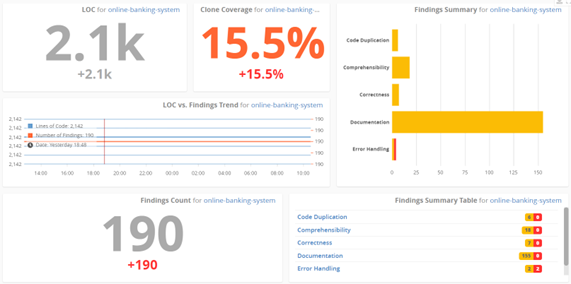
\includegraphics[width=13cm]{D1-Reengineering Opportunity/images/Picture1.png}
\caption{Code Quality Report of Online Banking System - TeamScale Dashboard}
\end{center}
\end{figure}
\pagebreak
\addcontentsline{toc}{subsection}{4.2. Currency Converter}
\subsection*{4.2. Currency Converter\hfill {\normalsize{Iphigenia Pappas - 40077089}}} \\
\normalsize {\textbf{Project Description:}} \\
\normalsize {Currency converter (or currency exchange) is a mini project coded in Java programming language. This simple application provides a web-based interface for exchanging/converting money from one currency to another currency. It is simply a calculator-like app developed using Ajax, Java servlets web features. In this application, there is regular update about currency of every country by which it displays present currency market value and conversion rate. Such application can be used by any user, but it is mainly useful for business, shares, and finance related areas where money transfer and currency exchange take place daily.}\\
\\
\normalsize{\textbf{System Source Code :}} \\
\normalsize{\  https://github.com/projectworldsofficial/currency-converter-in-java.git }\\
\\
\normalsize{\textbf{System Stack :}}\\
\normalsize{Java Servlets(Java), Ajax}\\
\\
\normalsize{\textbf{Repudiation Rationale : }}\\
\normalsize{This repository had many issues, however the large majority of things that stuck out were features that were not implemented properly. I noticed many defects. Firstly, on top of all the maintenance that needs to be done to the code, the bigger issue was a performance issue, this task could have been done in O(1) rather than O(n) by using a switch statement. The interface defects also bothered me, as much work could have been done to make it more user friendly and allow it to perform multiple conversions at once. There are also multithreading defects as we cannot execute multiple tasks at once. The problem with multithreading, however, is that sometimes there is the condition of deadlock where starvation is created, and if not handled and debugged properly, can end up leading to a failure of the system. Most of the issues had to do with the design of the software rather than the actual code itself, and as this is not the end goal of this assignment (to add enhancements and change the software) therefore we rejected this Software chosen.}
\\
\begin{figure}[htb]
\begin{center}
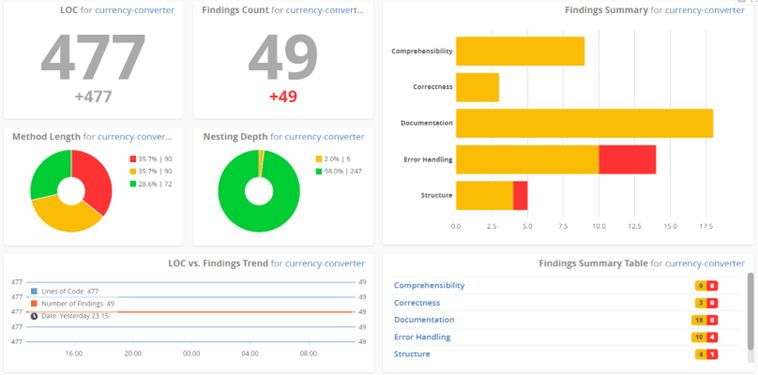
\includegraphics[width=12cm]{D1-Reengineering Opportunity/images/Picture2.png}
\caption{Code Quality Report of Currency Converter - TeamScale Dashboard}
\end{center}
\end{figure}
\pagebreak
\addcontentsline{toc}{subsection}{4.3. Hotel Management System}
\subsection*{4.3. Hotel Management System\hfill {\normalsize{Heet Patel - 40179213}}} \\
\normalsize {\textbf{Project Description:}} \\
\normalsize {Hotel Management System is developed in java platform. This is a Web Base Management System developed for Managing Hotel Day. This application covers all activities in the hotel including Registrations, Employee Management, Bill Printing, Account Control, Result analysing, Food and Beverage Details, and Issuing Rooms. The system role is divided into two types: manager (administrator) and employee (ordinary user), of which manager (administrator) has the right to view all bookings, delete rooms, view employees, add employees and other functional permissions Employees (ordinary users) have the right to view available rooms, customer reservations, modify reservations, delete reservations, register new customers and other functional permissions (tasks are self-drafted).}\\
\\
\normalsize{\textbf{System Source Code :}} \\
\normalsize{\ https://github.com/jsanhuo/HotelManagementSystem.git}\\
\\
\normalsize{\textbf{System Stack :}}\\
\normalsize{HTML5, CSS3, JavaScript, Bootstrap3, JDK1.8 + Spring Boot, Mybatis (Persistence Layer Framework), Druid (Database Connection Pool).}\\
\\
\normalsize{\textbf{Repudiation Rationale : }}\\
\normalsize{The Hotel Management System followed a similar structure as our chosen candidate, it was easily to categorize the system in two groups which includes manager (administrator) and employee (ordinary user). This system was also split into many different functionalities that have been listen in the paragraph above entitled Project Description. There were three particular reasons we rejected this system. Firstly it had far too many components and was difficult to follow, what made it even worse to follow is that the comments and documentation of the repository seem to have been done in a language that none of our team mates are familiar with. This makes it that much more difficult to follow the code. We also took into consideration that the number of undesirables was less than the chosen candidate. This was part of our reason for rejection, but certainly not the main one.}
\\
\begin{figure}[htb]
\begin{center}
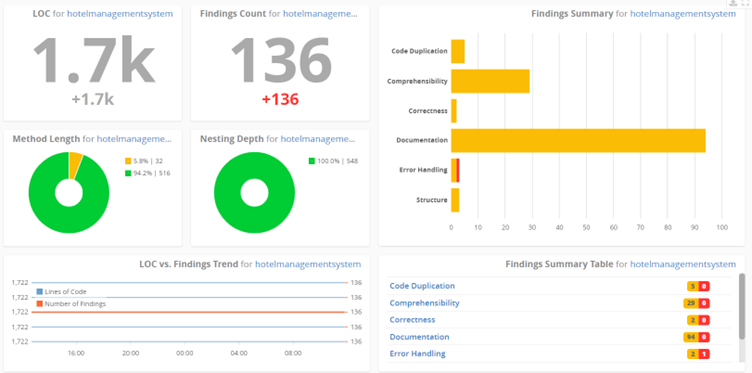
\includegraphics[width=12cm]{D1-Reengineering Opportunity/images/Picture3.png}
\caption{Code Quality Report of Hotel Management System - TeamScale Dashboard}
\end{center}
\end{figure}
\pagebreak
\addcontentsline{toc}{subsection}{4.4. Product Management System}
\subsection*{4.4. Product Management System\hfill {\normalsize{KevinKumar Patel - 40194915}}} \\
\normalsize {\textbf{Project Description:}} \\
\normalsize {It is a marketplace where customer can place order and Admin can manage inventory of products, view order and generate the report.}\\
\\
\normalsize{\textbf{System Source Code :}} \\
\normalsize{\ https://github.com/anantjain6/ProductManagementSystem.git}\\
\\
\normalsize{\textbf{System Stack :}}\\
\normalsize{Java 8, Spring MVC, Spring Data, Spring Boot, Hibernate JPA, H2 In-memory Database, Maven for Dependency Management.}\\
\\
\normalsize{\textbf{Repudiation Rationale : }}\\
\normalsize{The product management system was far too complex for the level of this course. Simply understanding the multiple technologies used that can be found below require more time to learn:\\
* Maven for Dependency Management\\
* Spring MVC for Web application development\\
* Spring Data JPA for Creating Custom Repository\\
* Spring Boot for Autoconfiguration\\
* Spring Security for Authentication & Authorisation\\
* Hibernate Validator for form data validation\\
* H2 In-memory Database for Storing data\\
* Java Mail API to send HTML E-Mail over SMTP\\
* JSTL\\
We want to concentrate our efforts in the maintenance of the code within the scope of this course, rather than spend countless hours trying to learn multiple new technologies. This would have complicated the end goal of this assignment and most importantly this course.}
\\
\begin{figure}[htb]
\begin{center}
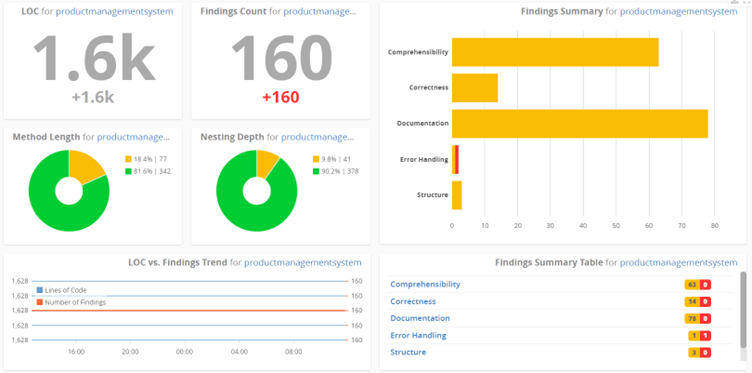
\includegraphics[width=13cm]{D1-Reengineering Opportunity/images/Picture4.png}
\caption{Code Quality Report of Product Management System - TeamScale Dashboard}
\end{center}
\end{figure}
\pagebreak
\addcontentsline{toc}{subsection}{4.5. E-book stall}
\subsection*{4.5. E-book stall\hfill {\normalsize{Venis Patel - 40170617}}} \\
\normalsize {\textbf{Project Description:}} \\
\normalsize {The application is built to create an online platform to sell books, The application comprises of functionalities like maintaining books selling history, adding, and managing books, updating the availability of books, filtering the books based on author or the publisher and the simulation of online payment method to buy the book. The application is built in Generic Servlets in Java, JDBC and MySQL.}\\
\\
\normalsize{\textbf{System Source Code :}} \\
\normalsize{\ https://github.com/shashirajraja/onlinebookstore.git}\\
\\
\normalsize{\textbf{System Stack :}}\\
\normalsize{\ Html, CSS, JavaScript, Java [JDK 8+], JDBC, Servlet, MySQL, Apache Maven.}\\
\\
\normalsize{\textbf{Repudiation Rationale : }}\\
\normalsize{\This project was well made, this exact project is often given in courses to test object oriented programming skills. Jenna had to make a project almost exactly like this one. However, that being said, the system was far too basic. It concentrates more on OOP than actually building a software. This surely also explains why the number of undesirables was far less than other projects, because it’s not nearly as complex as we would need it to be in order to apply multiple fixes. We also couldn’t find many undesirables, the main issues include changing the code for it to be better optimized, which is not the purpose of this assignment. Lastly, we also rejected this software because 50 percent of it was front end. It is far too much a surface level project for the scope of this course.}
\\
\begin{figure}[htb]
\begin{center}
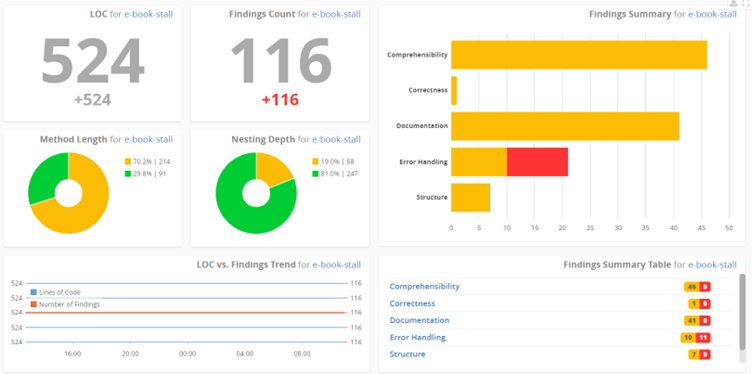
\includegraphics[width=13cm]{D1-Reengineering Opportunity/images/Picture5.png}
\caption{Code Quality Report of E-Book Stall - TeamScale Dashboard}
\end{center}
\end{figure}
\pagebreak
\addcontentsline{toc}{section}{5. Candidate System Descriptions}
\section*{5. Candidate System Description}
\normalsize {The Online Banking System is a banking portal on the web which manages the customer profile and manages their transactions. It is highly scalable and secured with the help of Spring Security. The main feature of this project is validation of login form, viewing customer profile, viewing transaction details of the customer ,Viewing balance of the customer, Approval of the changes in the address by the customer. The core objective of this project is to maintain a personal account in the bank. The system also provides the access to the customer to create an account, deposit/withdraw the cash from the account, also to view reports of all the accounts available. }\\

\addcontentsline{toc}{section}{6. Candidate System Rationale}
\section*{6. Candidate System Rationale}
\normalsize{The reason we chose the online banking system as our candidate system is not only because it was the better one of the choices from the software provided by the team (rejected reasons can be found below for all other systems) but for several other important reasons. To name a few, this system met all the requirements and more. This was complex enough and for us to have a lot to work on, without being too much where we would get lost in the code. There is not too much spaghetti code, although it may be optimized to less lines of code. This project was between 1000 to 2000 lines of code which was the target desire for our system. We also were easily able to locate the 25 undesirables to fix for this system, each team member was able to identify 5 distinct undesirables that we can easily distribute to the team to provide a fix. Lastly, this system was written in large majority in our programming language of choice which is Java. The architecture of this system also contains multiple distinct aspects that we can easily categorize in two main groups: managing customer profile and managing transactions. This system also contains a certain level of security as it maintains credential information by validating a log in form. This, then allows us to do other actions such as viewing customer profile, viewing transaction details of the customer, viewing balance of the customer, approval of the changes in the address by the customer. In summary, this system met all the requirements and more and was well structured enough for us to clearly identify our undesirables.}\\
\begin{figure}[htb]
\begin{center}
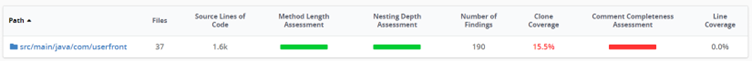
\includegraphics[width=13cm]{D1-Reengineering Opportunity/images/Picture6.png}
\caption{overall assessment generated for Candidate R online banking system from TeamScale}
\end{center}
\end{figure}

\begin{figure}[htb]
\begin{center}
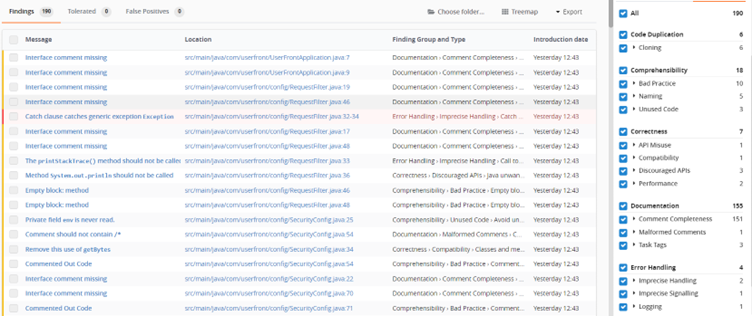
\includegraphics[width=13cm]{D1-Reengineering Opportunity/images/Picture7.png}
\caption{Category of Findings generated for Candidate R online banking system from TeamScale}
\end{center}
\end{figure}

\begin{figure}[htb]
\begin{center}
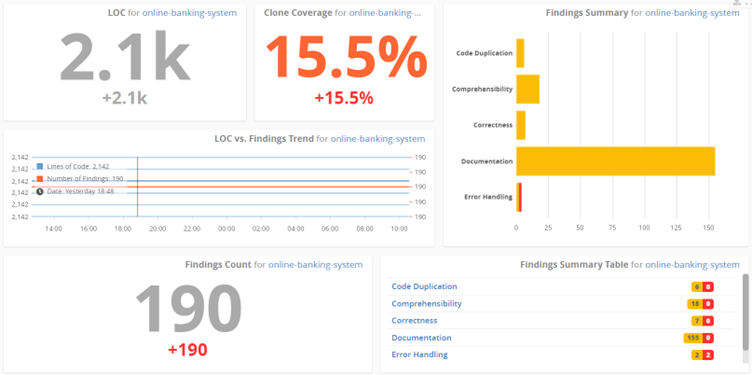
\includegraphics[width=10cm]{D1-Reengineering Opportunity/images/Picture9.png}
\caption{Code Quality Report of Online Banking System - TeamScale Dashboard}
\end{center}
\end{figure}

\begin{figure}[htb]
\begin{center}
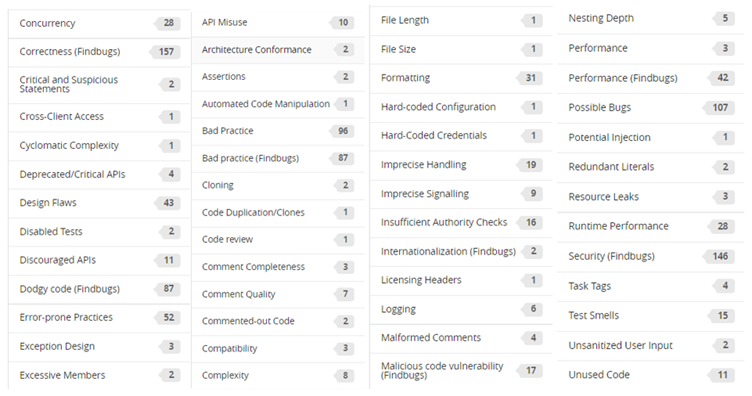
\includegraphics[width=10cm]{D1-Reengineering Opportunity/images/Picture8.png}
\caption{Quality Metrics used to assess Candidate R online banking system from TeamScale}
\end{center}
\end{figure}

\clearpage
\addcontentsline{toc}{section}{7. References}
\section*{7. References}
 \href{https://www.quora.com/How-do-you-define-code-quality}{1. D. Korolev, "How do you define code quality?," 09 02 2014. [Online].}.\\
 \href{http://www.iso.org/iso/catalogue_detail.htm?csnumber=35733}{2. ISO/IEC 25010:2011," 03 2011. [Online]. }.\\
 \href{http://www.iso.org/iso/catalogue_detail.htm?csnumber=22749}{3. ISO/IEC 9126-1:2001," 06 2001. [Online]}.\\
 \href{http://www.w3schools.com/xml/}{XML Tutorial," 2017. [Online].}.\\
 \href{http://stackoverflow.com/questions/872103/what-is-the-optimal-size-of-a-software-develo}{4. What is the optimal size of a software development team," 16 05 2009. [Online].}.\\
 \normalsize{5. R. &. Norvig, The intelligent agent paradigm, 2003, pp. 27, 32–58, 968–972 .}\\
  \href{https://docs.teamscale.com/#why-teamscale-is-different.}{6. "Teamscale Documentation" [Online].}.\\
\end{document}
